%
%  untitled
%
%  Created by vbosch on 2011-02-07.
%  Copyright (c) 2011 McBosch. All rights reserved.
%
\documentclass[a4paper,10pt,titlepage]{article}

% Use utf-8 encoding for foreign characters
\usepackage[utf8]{inputenc}

% Setup for fullpage use
\usepackage{fullpage}
\usepackage{titlepic}
\usepackage{float}
\usepackage{color}

% Uncomment some of the following if you use the features
%
% Running Headers and footers
%\usepackage{fancyhdr}

% Multipart figures
%\usepackage{subfigure}

% More symbols
\usepackage{amsmath}
%\usepackage{amssymb}
%\usepackage{latexsym}

% Surround parts of graphics with box
\usepackage{boxedminipage}

% Package for including code in the document
\usepackage{listings}

% If you want to generate a toc for each chapter (use with book)
\usepackage{minitoc}

% This is now the recommended way for checking for PDFLaTeX:
\usepackage{ifpdf}

%\newif\ifpdf
%\ifx\pdfoutput\undefined
%\pdffalse % we are not running PDFLaTeX
%\else
%\pdfoutput=1 % we are running PDFLaTeX
%\pdftrue
%\fi

\ifpdf
\usepackage[pdftex]{graphicx}
\else
\usepackage{graphicx}
\fi
\title{Advances in Neural Networks \\ Course Project - Terrain Classification}
\author{Vicente Bosch Campos \dag \\
\textcolor{blue}{\texttt{viboscam@posgrado.upv.es}}}
\titlepic{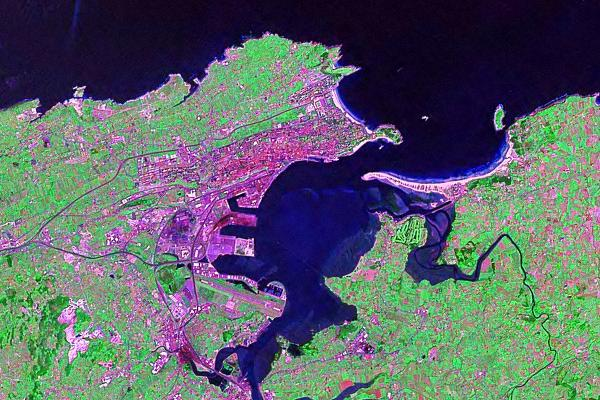
\includegraphics[width=250pt]{cover.jpg}}

\date{\today}

\begin{document}

\ifpdf
\DeclareGraphicsExtensions{.pdf, .jpg, .tif}
\else
\DeclareGraphicsExtensions{.eps, .jpg}
\fi

\maketitle

\tableofcontents

\listoffigures

\section{Introduction}

\par The application of Support Vector Machines to uni - dimensionally multi-spectral representation of a 3x3 pixel matrix of an image section to recognize terrain type of the central pixel is considered in this course project.
\\
\par The use of Pattern Recognition and Image Analysis is quite established for the task of satellite image classification. In this course project we consider the classification of terrain types.


\subsection{Data}

\par A Landsat MSS image consists of four digital images of the same zone using different spectral bands. Two of the bands are in the visible region (corresponding approximately to green and red regions of the visible spectrum) while the other two are in the (near) infra-red. Each pixel is represented as a 8-bit binary word, with 0 corresponding to black and 255 to white. The spatial resolution of a pixel is approximately 80m x 80m. Each image contains 2340 x 3380 such pixels.
\\
\par The database used in the course project is a sub-area of a scene, consisting of 82 x 100 pixels. Each line of data corresponds to a 3x3 square neighborhood of pixels completely contained within the 82x100 sub-area. Each line contains the pixel values in the four spectral bands (converted to ASCII) of each of the 9 pixels in the 3x3 neighborhood and a number indicating the classification label of the central pixel. As per the original database the number is a code for the following classes:
\begin{enumerate}
	\item red soil
	\item cotton crop
	\item grey soil
	\item damp grey soil
	\item soil with vegetation stubble
	\item mixture class ( all types present)
	\item very damp grey soil
\end{enumerate}

\par Further preprocessing has been performed to the data provided to us. It has been normalized and as there are no records of the 6th type the classes label have been moved so that type 7 is represented by the label 6. 

\par We have been provided with two data partitions:
\begin{itemize}
	\item sat6c.tra: Training set formed by 2000 records with the following composition:	
	\begin{itemize}
		\item Class 1: 466
		\item Class 2: 216
		\item Class 3: 429
		\item Class 4: 195
		\item Class 5: 226
		\item Class 6: 468
	\end{itemize}
	\item sat6c.public.tst: Public test set containing of 1000 records with the following composition: 
	\begin{itemize}
		\item Class 1: 234
		\item Class 2: 106
		\item Class 3: 208
		\item Class 4: 98
		\item Class 5: 118
		\item Class 6: 236
	\end{itemize}
\end{itemize}


\subsection{Scope}

\par As part of the course project we will train classifiers for the landstat task described in the above sections. To be more precise we will use the following techniques:
\begin{itemize}
	\item Support Vector Machines:
		\begin{itemize}
			\item Multi class algorithm 
			\item Combination of two class classifier
		\end{itemize}
	\item For both SVM techniques we will use the following Kernels:
	\begin{itemize}
		\item Polynomial Kernel: \begin{math} (\ s\ a*b +c)^d\end{math}
		\item Radial Basis Function Kernel: \begin{math} exp(\ -gamma\ ||a-b||^2) \end{math}
		\item Sigmoid Kernel: \begin{math} tanh(\ s\ a*b + c) \end{math}		
	\end{itemize}
\end{itemize}

\par All training classification will be performed with the sat6c.tra data and the best obtained classifiers will be evaluated against the sat6c.public.tst data set, which is not used for training nor for partial evaluation/guidance of the performance during the experimentation. 

\section{Development}

\par In this section we will describe the software framework developed in order to perform the experimentations for the task. The framework developed allows us to load, format and perform transformations with specific data sets and also launch classifier training with different classifiers and obtain mean test set classification error with cross validation. 

\subsection{Software Structure}

\par The software is structured into the following classes:
\begin{description}
	\item[DataPattern:] The DataPattern class is defined in the \textit{./lib/data\_pattern.rb} file. It encapsulates a sample record of class containing the actual data ( can be in numeric or string representations) and the class label. It allows us to perform the following operations: 
	\begin{itemize}
		\item Order to records by label value.
		\item Iterate over the different values of the vector.
		\item Duplicate the record.
	\end{itemize}
	\item[DataSet:] The DataSet class can be found in the \textit{./lib/data\_set.rb} file. It represents a whole set of records of a task allowing us to perform the following tasks over them:
	\begin{itemize}
		\item Read the original data from a file and apply specific format to them to prepare them for the ML tool. e.g. Uniform the chain length for a Chromosome classification task. 
		\item Write them to file using an specific format for a Machine Learning toolset.
		\item Partition the set into blocks ensuring correct representation and number of each class in the block.
		\item Combine different sets in an additive manner.
		\item Sort the set by class label.
		\item Shuffle the set.
		\item Filter the set to a sub set of labels/classes.
		\item Binarize labels so that they can be sent to 2-class limited classifiers. 
	\end{itemize}
	\item[Snns:] The Snns class can be found in the \textit{./lib/snns.rb} file. It is an object wrapper for the Batchman snns interface and allows us to perform the following tasks from the framework:
	\begin{itemize}
		\item The class allows as input an experiment object, it automatically generates an specific batchman script file and runs it. 
		\item Permits us to programmatically access to the results of the .res files when reviewed with the analyze tool.
	\end{itemize}
	\item[SnnsFileWriter:] The SnnsFileWriter class can be found in the \textit{./lib/snns.rb} file. The file writer is in charge of performing header and footer special formatting for the toolset chosen. In this case it allows us to call mkhead from the framework to prepare the pattern files. 
	\item[SnnsPatternWriter:] It can be found in \textit{./lib/snns.rb}. The pattern writer in in charge of performing special formatting to the patterns required for correct usage on the desired toolset. In this case it ensures there is a space between each dimension value and ensures there is a line space between the vector and the class label. 
	\item[Parameter:] Coded in \textit{./lib/parameter.rb}. The class allows us to define a parameter and a range of values of variation. The values can be a set of strings, if for example we want to vary between different neural network files or a numeric value, to study an specific range of the momentum parameter. 
	\item[Experiment:] Present in the file \textit{./lib/experiment.rb}. It is an specific configuration, value set, of the parameters that will be executed on the chosen ML tool set and the value will be averaged over cross experimentation. 
	\item[Study:] contained in \textit{./lib/study.rb}. It generates the set of experiments by performing combinations of each of the values for each parameter described and runs them writing the results and studies performed in specific files. 
\end{description}
\subsection{Library Options}

\par With the defined software structure we can easily perform studies on an indicated task by just having to write the specific
read and write formatters for the task. Next we will show a short example of the framework scripts used to train neural networks 
for the chromosome classification task: 

\lstset{basicstyle=\footnotesize,language=Ruby}
\lstset{linewidth=500pt}
\lstset{numbers=left, stepnumber=1}
\lstset{commentstyle=\color{blue}, stringstyle=\color{green},showspaces=false}
\lstset{keywordstyle=\color{red}\bfseries\emph}
\lstset{frame=trBL,frameround=tttt}
\lstinputlisting[caption=chromosome.rb,label=lst:lowertri]{../bin/svm_comb.rb}

\subsection{Software Output}

\par The software generates the following output files that will help us out for the review of the classification training:

\begin{description}
	\item[Study List:] Is a detailed print out indicating the parameters used in the experiment as well as the pattern files and output files in case the experiment wants to be reviewed in detail:
	{\footnotesize\begin{verbatim}
______________________________________________________________________________________
1
{:algo=>"Quickprop", :in_model=>"../test/theory_data/trr_36_20_6.net", :learning=>0.15000000000000002, :max_growth=>0.1, 
:id=>1, :test_pat=>"./QP30_20_6/20110209-000607_test.pat", :val_pat=>"./QP30_20_6/20110209-000607_val.pat", 
:train_pat=>"./QP30_20_6/20110209-000607_train.pat", :out_model=>"./QP30_20_6/20110209-000607Quickprop.net", 
:test_res=>"./QP30_20_6/20110209-000607test.res", :val_res=>"./QP30_20_6/20110209-000607val.res"}
______________________________________________________________________________________
	\end{verbatim}}
	
	\item[Result File:] For each of the parameter combinations a result is printed out containing the mean error, wrong and right classification \% for the validation and test set over the cross training.
	\item[Log files:] Contains an execution log of the Batchman execution with the training and validation MSE.
	\item[Bat files:] Automatically generated Batchman script for the experiment.
	\item[Snns standard files:] It also generates and saves the following SNNS files:
	\begin{itemize}
		\item Result files of the validation and test sets.
		\item Pattern files used in the training.
		\item Resulting neural network.
	\end{itemize}
\end{description}


\section{Experimental Results}
\subsection{Neural Networks}


\section{Conclusions}

\par As we have seen in the previous tasks the best results have been obtained for the Radial based learning. The best results for each algorithm in the private test set has been as follows: 

\begin{table}[H] 
\caption{Private test set - best error results for training algorithms} %title of the table
\centering 
\begin{tabular}{c c c} 
\hline\hline 
Back-propagation & Quick-propagation & Radial Network \\
10.40 & 15.50 &  9.60 \\

\hline 
\end{tabular} 
\label{tab:dist_result} 
\end{table}

\par We have obtained the best results for Back-propagation and Radial based learning, being our radial network the network with least classification task in the board.

\par In future work it would be interesting to use the SVM software that has been integrated in the framework to study this task.  

\end{document}
